\documentclass[12pt,a4paper]{report}

\usepackage[utf8]{inputenc}
\usepackage[spanish]{babel}
\usepackage[left=3cm,right=3cm,top=3cm,bottom=3cm]{geometry}
\usepackage{graphicx}
\usepackage{amsmath}
\usepackage{amsfonts}
\usepackage{hyperref}
\usepackage{xcolor}
\usepackage{minted}

\title{Reporte proyecto 1}
\author{Bruno Bernardo Soto Lugo}
\date{\today}

\begin{document}

\thispagestyle{empty}

\begin{figure}[ht]
  \minipage{0.76\textwidth}
  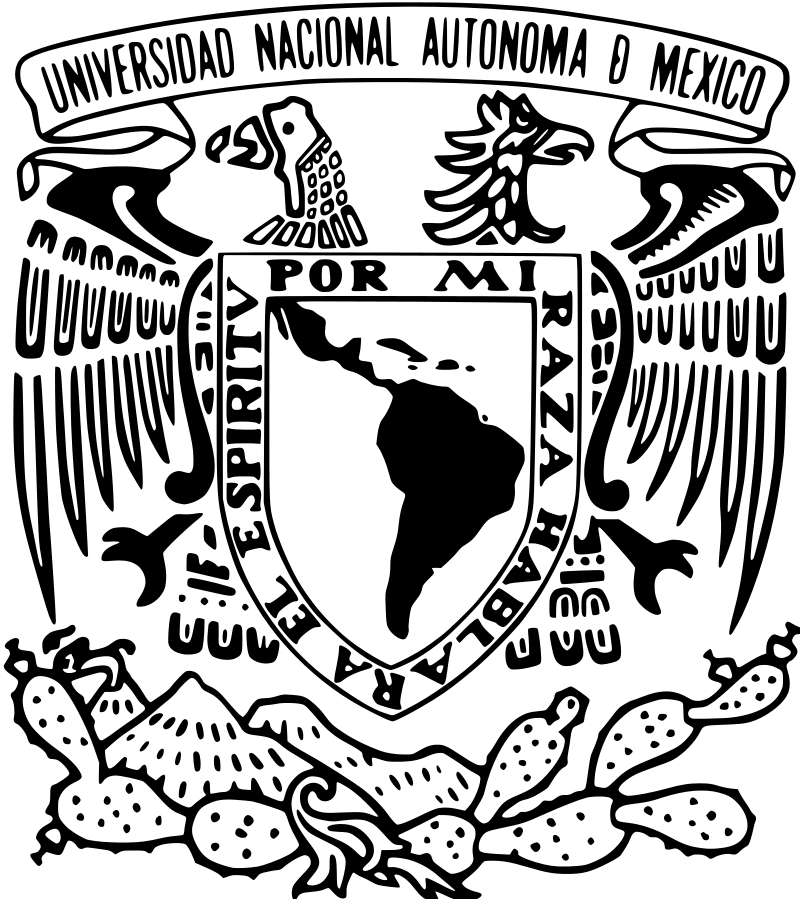
\includegraphics[width=4cm]{logo_unam.png}
  \label{EscudoUNAM}
  \endminipage
  \minipage{0.32\textwidth}
  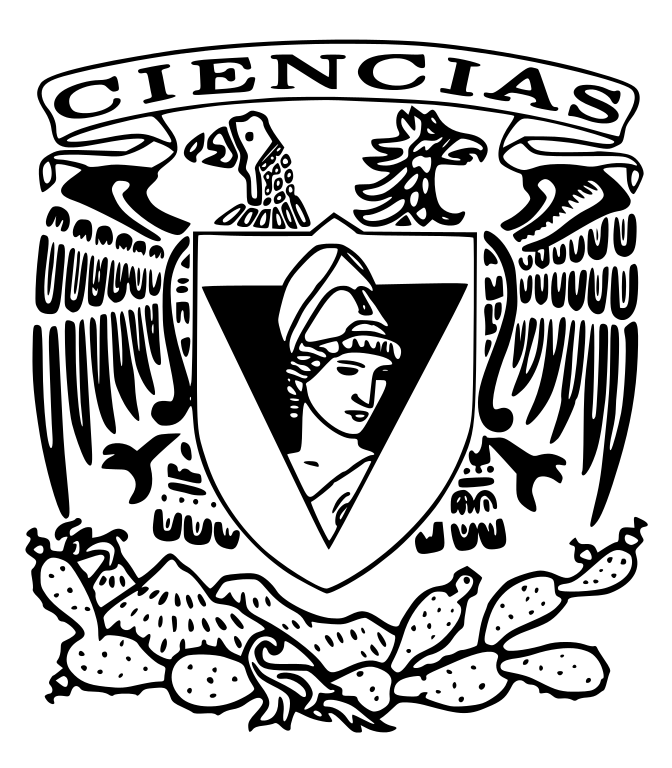
\includegraphics[height=4.9cm, width=4cm]{logo_ciencias.png}
  \label{EscudoFC}
  \endminipage
\end{figure}

\begin{center}
	\vspace{0.8cm}
	\LARGE
	UNIVERSIDAD NACIONAL AUTÓNOMA DE MÉXICO
  
	\vspace{0.8cm}
	\LARGE
  FACULTAD DE CIENCIAS
  
	\vspace{1.7cm}
	\Large
	\textbf{Reporte proyecto 1 (Implementación de protocolo de chat utilizando sockets TCP).}
  
	\vspace{1.3cm}
	\normalsize
	PRESENTA \\
	\vspace{.3cm}
	\large
	\textbf{Bruno Bernardo Soto Lugo \\ 426008646}
  
	\vspace{1.3cm}
	\normalsize
	PROFESOR \\
	\vspace{.3cm}
	\large
	\textbf{Canek Peláez Valdés} \\

	\vspace{1.3cm}
	\normalsize
	AYUDANTES \\
	\vspace{.3cm}
	\large
	\textbf{Miriam Torres Bucio} \\
	\textbf{Cynthia Lizbeth Sánchez Urbano} \\
  
\end{center}

\newpage

\tableofcontents

\newpage

\chapter{Introducción}
El presente documento detalla el proceso de implementación de un protocolo que especifica una forma de comunicación chat. El sistema está compuesto por dos componentes principales: un cliente con interfaz gráfica desarrollado en \textbf{Kotlin} con el framework \textbf{Compose Multiplatform} y un servidor desarrollado en lenguaje \textbf{C}. 

El objetivo principal del proyecto es implementar un protocolo de comunicación basado en objetos JSON que permita la identificación de usuarios, cambio de estados (Activo, Ausente, Ocupado), envío de mensajes privados y públicos, así como la gestión de salas de chat dinámicas. El desarrollo siguió el modelo de cascada.

Las etapas fueron:
\begin{enumerate}
    \item \textbf{Análisis:} Definición de requisitos funcionales basados en las acciones del usuario.
    \item \textbf{Diseño:} Arquitectura del sistema, diseño de la base de datos en memoria y diagramas UML.
    \item \textbf{Desarrollo:} Codificación del servidor en C y la interfaz en Kotlin.
    \item \textbf{Pruebas:} Validación de cada comando del protocolo contra el manual de especificaciones.
\end{enumerate}

\chapter{Análisis}
En esta fase se definieron las capacidades que la implementación del sistema debe ofrecer según el protocolo.

\section{Requisitos}
A partir del análisis del protocolo, se identificaron los siguientes componentes:

\begin{itemize}
  \item \textbf{Gestión de Identidad (IDENTIFY):} El sistema debe permitir al usuario unirse con un nombre único (con máximo 8 caracteres). El servidor debe validar la existencia previa y notificar a otros usuarios la entrada de nuevos miembros.
  \item \textbf{Gestión de Estado (STATUS):} Los usuarios pueden alternar entre \textbf{ACTIVE}, \textbf{AWAY} y \textbf{BUSY}. Cada cambio debe disparar un evento \textbf{NEW\_STATUS} para los demás clientes conectados.
  \item \textbf{Comunicación (TEXT, PUBLIC\_TEXT y ROOM\_TEXT):} 
        \begin{itemize}
          \item Mensajes privados que solo el destinatario recibe.
          \item Mensajes públicos dirigidos a todos los usuarios en la conexión global.
          \item Mensajes dirigidos a todos los usuarios en una sala.
        \end{itemize}
  \item \textbf{Gestión de Salas (ROOMS):} El sistema debe permitir crear salas (con máximo 16 caracteres), invitar usuarios y gestionar pertenencia a sala. Se requiere validación de que el usuario esté invitado antes de unirse.
  \item \textbf{Obtención de usuarios (USERS y ROOM\_USERS):} El usuario puede obtener la lista de usuarios que están conectados globalmente o en una sala a la que pertenece.
  \item \textbf{Desconexión (DISCONNECT):} Manejo de limpieza de recursos cuando un cliente pierde conexión o decide salir, notificando su salida a las salas que pertenece y globalmente.
\end{itemize}

\begin{figure}[H]
  \centering
  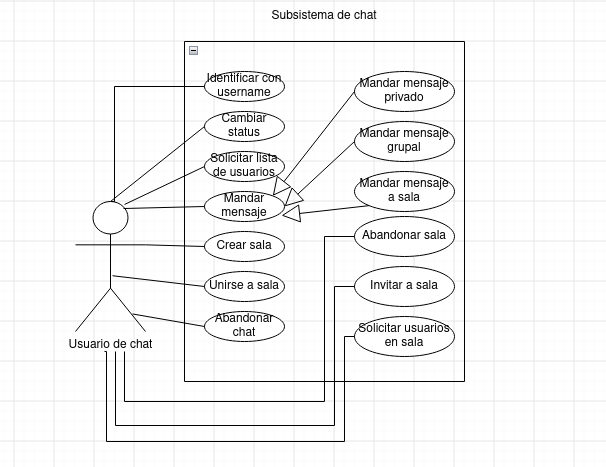
\includegraphics[width=8cm]{Analisis_drawio.png}
  \caption{Diagrama del análisis (Use Case).}
\end{figure}

\chapter{Diseño}
El diseño implementa una arquitectura dividida en cliente y servidor con el objetivo de desacoplar las partes del programa y permitir que diferentes clientes puedan conectarse a un mismo servidor. El servidor actúa como un gestionador de múltiples conexiones simultaneas. El cliente se encarga de la representación visual y la administración de la lógica local.

\section{Diagramas UML}
A continuación se detallarán en diagramas UML las estructuras usadas para implementar el protocolo.

\subsection{Diagrama de secuencia (Proceso de autenticación)}
El siguiente diagrama representa la secuencia que sigue el cliente y el servidor cuando un usuario busca autenticarse. 

% Código de plantUML
%@startuml
%actor Cliente
%participant "Hilo de conexión" as Hilo
%participant "Administrador de autenticación" as Auth
%database "Lista de usuarios (global)" as Global
%
%Cliente -> Hilo : {"type":"IDENTIFY","username":"A"}
%Hilo -> Auth : Iniciar autenticación
%Auth -> Auth : Decodificar JSON
%Auth -> Global : Añadir usuario
%alt usuario nuevo
   %Global --> Auth : true
   %Auth -> Global : Obtener registro de usuario (Para futuras operaciones)
   %Auth -> Cliente : RESPONSE IDENTIFY SUCCESS
   %Auth -> Global : Enviar mensaje a otros usuarios.
   %Global --> "otros clientes" : NEW_USER {username: "A"}
%else usuario ya existía
   %Global --> Auth : false
   %Auth -> Cliente : RESPONSE IDENTIFY USER_ALREADY_EXISTS
%end
%@enduml

\begin{figure}[H]
  \centering
  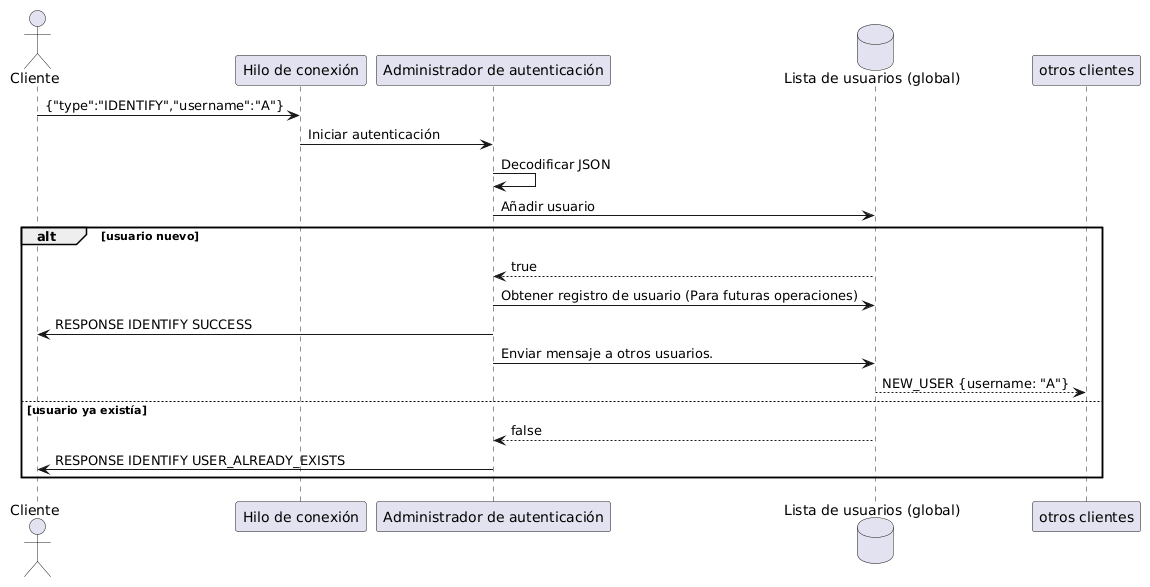
\includegraphics[width=13cm]{Secuencia_Auth.png}
  \caption{Diagrama de la autenticación.}
\end{figure}

\chapter{Desarrollo}

\end{document}
